\subsection{Anwendung und Test}
Um die Implementierungen der Schnittstellen zur ArangoDB zu testen, werden die beiden Webservices (Java und FOXX) abgefragt. Das Frontend kann unter folgendem Link im Cluster erreicht werden: \texttt{http://10.20.110.61/team38/sdb-foxx-service/}


Um zufällige Schwankungen abzufangen, werden bei jeden Szenario mehrere Requests gemacht und ein Durchschnittswert ermittelt. Die Tests der Anwendungsszenarien werden mit jeweils 100 Anfragen getestet. Daraus ergeben sich dann folgende Ergebnisse:


\begin{figure}[htbp] 
  	\centering
     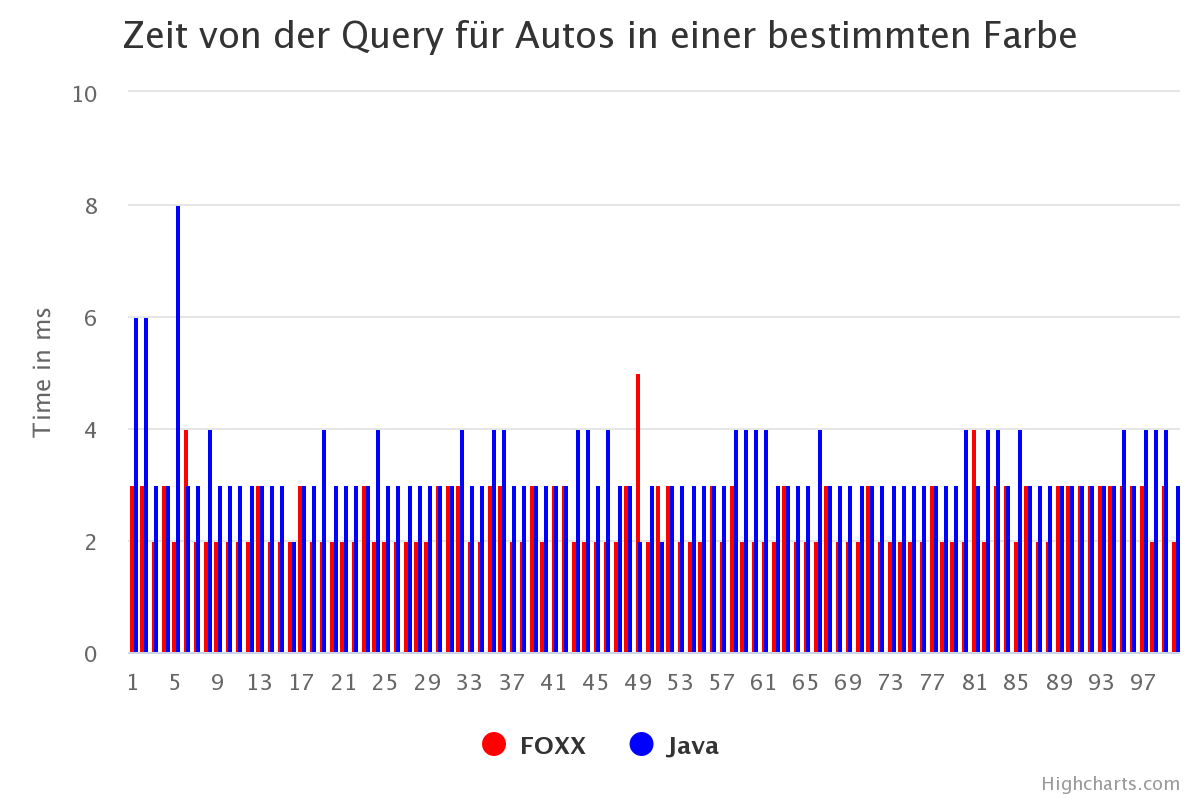
\includegraphics[width=1\textwidth]{./images/8.UseCase1Diagramm.png}
 	\caption{Anwendungsszenario 1 Ergebnisse}
  \label{fig:DataSchema}
\end{figure}


\begin{figure}[htbp] 
  	\centering
     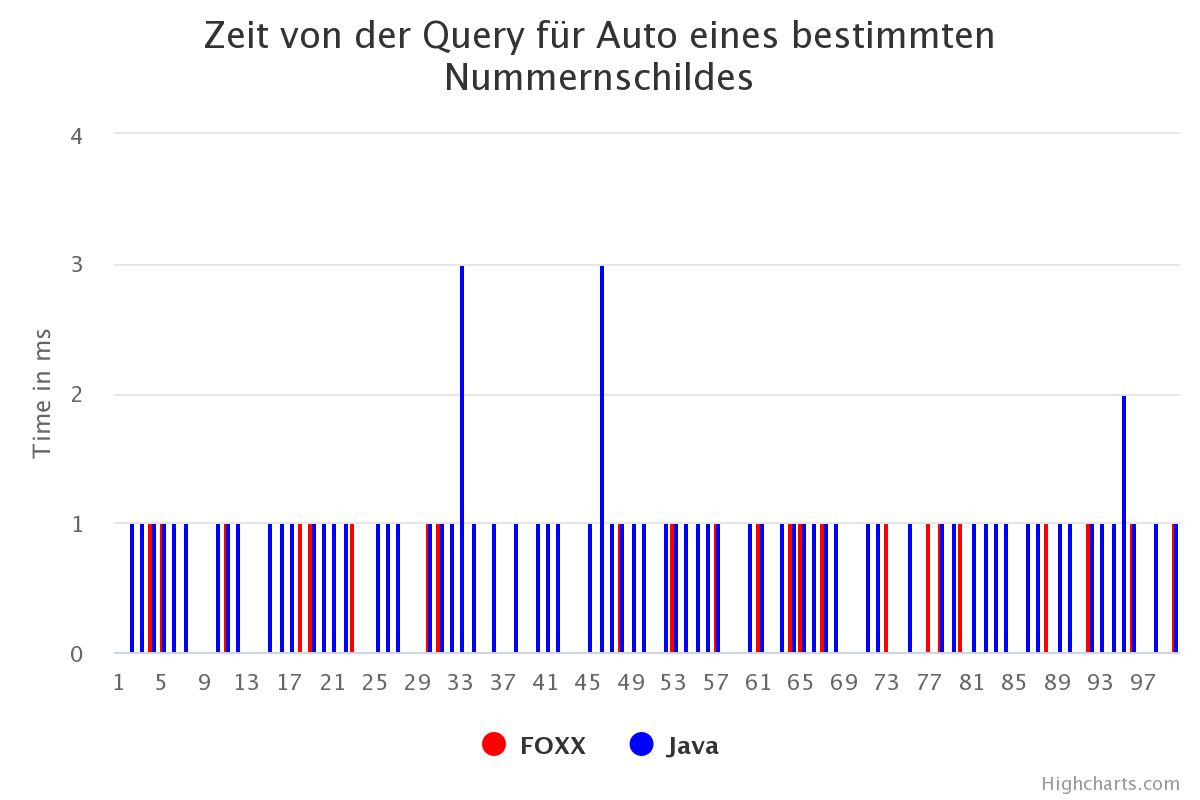
\includegraphics[width=1\textwidth]{./images/8.UseCase2Diagramm.png}
 	\caption{Anwendungsszenario 2 Ergebnisse}
  \label{fig:DataSchema}
\end{figure}


\begin{figure}[htbp] 
  	\centering
     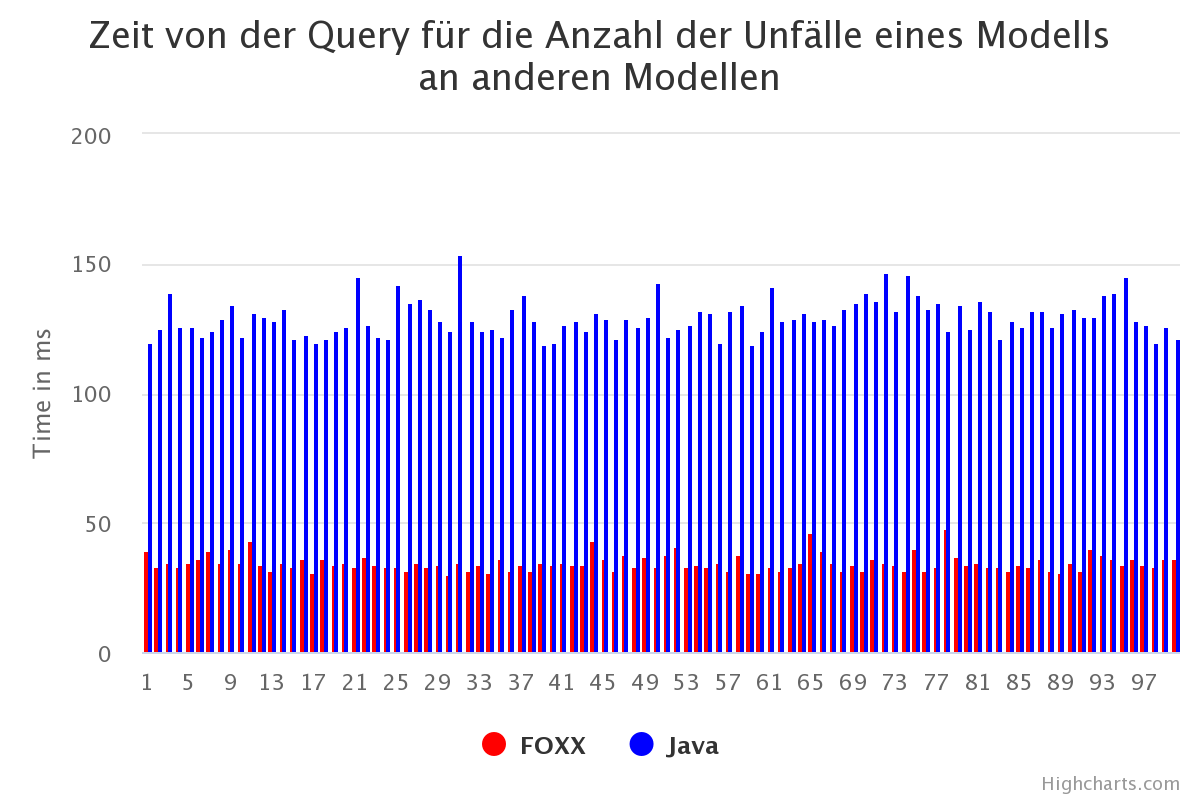
\includegraphics[width=1\textwidth]{./images/8.UseCase3Diagramm.png}
 	\caption{Anwendungsszenario 3 Ergebnisse}
  \label{fig:DataSchema}
\end{figure}